\documentclass[]{article}
\usepackage[utf8]{inputenc}

%Cosas de tikz necesarias
\usepackage{tikz}
\usetikzlibrary{positioning,arrows.meta}

\title{Practica TIKZ}
\author{Julian Zylber}
\date{October 2020}

\begin{document}

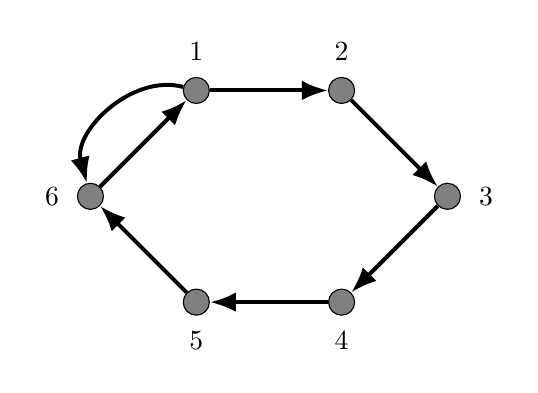
\begin{tikzpicture}[scale = 1,every node/.style={draw,circle,fill=gray}] %Opciones tikz para q los nodos sean un circulo relleno gris, y la escala
    %Los nodos son los nodos del grafo (duh!)
    %La sintaxis es \node[opciones] (nombre del nodo) {cosa q va adentro del nodo};
    %Se le puede poner labels si quieren, el manual de tikz es largo pero es excelente. Yo los puse para q la pasen mejor utds para entender el codigo
    
    \node[label={1}] (1) at (0,0) {}; %Este es el nodo llamado "1" q es un circulo de relleno gris
    \node[label={2},right= 15mm of 1] (2) {}; %Bellas referencias relativas
    \node[label=right:{3},below right= 11mm and 11mm of 2] (3) {};
    \node[label=below:{4},below left= 11mm and 11mm of 3] (4) {};
    \node[label=below:{5},left= 15mm of 4] (5) {};
    \node[label=left:{6},above left= 11mm and 11mm of 5] (6) {};
    
    %Bellos caminos (también relativos!)
    %GUARDA CON SPANISH BABEL ROMPE LAS FLECHAS (hay un fix preguntenmelo)
    \draw[line width=0.5mm,-Latex] (1) to (2); %El -Latex esla flecha
    \draw[line width=0.5mm,-Latex] (2) to (3);
    \draw[line width=0.5mm,-Latex] (3) to (4);
    \draw[line width=0.5mm,-Latex] (4) to (5);
    \draw[line width=0.5mm,-Latex] (5) to (6);
    \draw[line width=0.5mm,-Latex] (6) to (1);
    
    %Y una fancy para que vean q la rompe tikz
    \draw[line width=0.5mm,-Latex] (1)  to [bend right=60] (6);
    
    
    
\end{tikzpicture}

\end{document}
